\subsection{Modeling sequences: A brief overview}
\begin{itemize}
	\item When applying machine learning to sequences, we often want to turn an input sequence into an output sequence that lives in a different domain
	\begin{itemize}
		\item e.g., turn a sequene of sound pressures into words
	\end{itemize}

	\item When there is no separate target sequence, we can get a teaching signal by trying to predict the next term in the input sequence
	\begin{itemize}
		\item The target ouput sequence is the input sequence with and advance of 1 step
		\item This seems much more natural than trying to predict one pixel in an image from the other pixels, or one patch of an image from the rest of the image
		\item For temporal sequences there is a natural order for the predictions
	\end{itemize}

	\item Predicting the next term in a sequence blurs the distinction between supervised and unsupervised learning
	\begin{itemize}
		\item It uses methods designed for supervised learning, but it doesn't require a separate teaching signal (unsupervised)
	\end{itemize}

	\subsubsection{Memoryless models for sequences}
	\item \textbf{Autoregressive models}: predict the next term in a sequence from a fixed number of previous terms using ``delay taps.''
	\begin{center}
		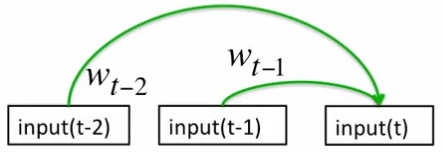
\includegraphics[scale=0.7]{sections/7/autoreg.png}
	\end{center}

	\item \textbf{Feed-forward neural nets}: generalize autoregressive models by using one or more layers of non-linear hidden units (e.g., Bengio's first language modle)
	\begin{center}
		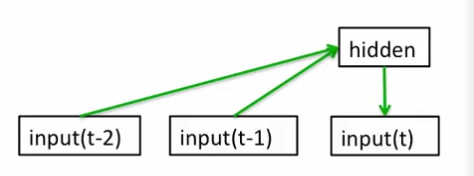
\includegraphics[scale=0.7]{sections/7/ffnn.png}
	\end{center}

	\subsubsection{Beyond memoryless models}
	\item If we give our generative model some hidden state, and if we give this hidden state its own internal dynamics, we get a much more interesting kind of model
	\begin{itemize}
		\item It can store information in its hidden state for a long time
		\item IF the dynamics is noisy and the way it generates outputs from its hidden state is noisy, we can never know its exact hidden state
		\item The best we can do is to infer a probability distribution over the space of hidden state vectors
	\end{itemize}
	\item This inference is only tractable for two types of hidden state model

	\subsubsection{Linear Dynamical Systems}
	\item These are generative models. They have a real-valued hidden state that cannot be observed directly.
	\begin{itemize}
		\item The hidden state has linear dynamics with Guassian noise and produces the observations using a linear model with Gaussian noise.
		\item There may also be driving inputs
	\end{itemize}
	\item To predict the next ouput (so that we can shoot down the missile) we need to infer the hidden state
	\begin{center}
		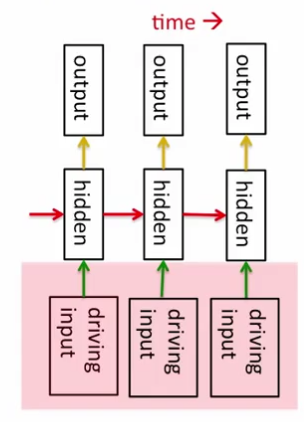
\includegraphics[scale=0.7]{sections/7/lds.png}
	\end{center}
	
	\subsubsection{Hidden Markov Models}
	\item HMM have a discrete one-of-N hidden state. Transitions between states are stochastic and controlled by a transition matrix. The outputs produced by a state are stochastic.
	\begin{center}
		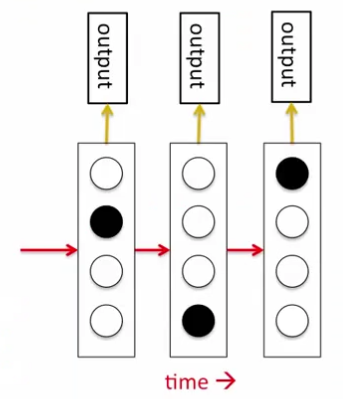
\includegraphics[scale=0.7]{sections/7/hmm.png}
	\end{center}
	\begin{itemize}
		\item We cannot be sure which state produced a given output. So the state is ``hidden.''
		\item IT is easy to represent a probability distribution across N states with N numbers
	\end{itemize}
	\item To predict the next ouput we need to infer the probability distribution over hidden states
	\item HMMs have efficient algorithms for inference and learning
	\item Fundamental limitation: consider what happens when a HMM generates data
	\begin{itemize}
		\item At each time step it must select one of its hidden states. So with N hidden states it can only remember log(N) bits about what it generated so far
	\end{itemize}
	\item Consider the information that the first half of an utterance contains about the second half
	\begin{itemize}
		\item The syntax needs to fit (e.g., number and tense)
		\item The semantics and intonation needs to fit
		\item The accent, rate, volume, and vocal tract characteristics must all fit 
	\end{itemize}
	\item All of these aspects combined could be 100 bits of information that's huge! 

	\subsubsection{Recurrent neural networks}
	\item RNNs are very powerufl, because they combine two properties
	\begin{itemize}
		\item Distributed hidden state that allows them to store a lot of information about the past efficiently
		\item Non-linear dynamics that allows them to update their hidden state in complicated ways
	\end{itemize}
	\begin{center}
		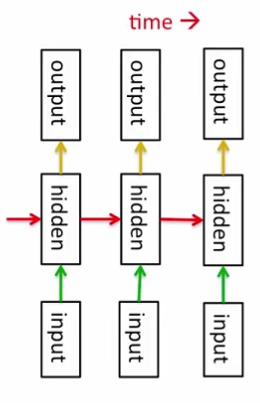
\includegraphics[scale=0.7]{sections/7/rnn.png}
	\end{center}
	\item With enough neurons and time, RNNs can compute anything that can be computed by your computer
	\item WHat kinds of behaviour can RNNs exhibit?
	\begin{itemize}
		\item They can oscillate (good for motor control)
		\item They can settle to point attractors (retrieving memories)
		\item Behave chaotically (bad for information processing)
		\item RNNs could potentially learn to implement lots of small programs that each capture a nugget of knowledge and run in parallel, interacting to produce very complicated effects
	\end{itemize}
	\item Computational power of RNNS make them very had to train
	\item 


	\subsubsection{Do generative models need to be stochastic?}
	\item LDS \& HMM are stochastic
	\begin{itemize}
		\item The posterior probability distribution over the hidden states given the observed data so far is a deterministic function of the data
	\end{itemize}
	\item RNN are deterministic
	\begin{itemize}
		\item So think fo the hidden state of an RNN as the equivalent of the deterministic probability distribution over hidden states in a LDS or HMM
	\end{itemize}

\end{itemize}

\subsection{Training RNNs with backpropagation}
\begin{itemize}
	\item The recurrent net is just a layered net that keeps reusing the same weights.
	\item Layered feedforward network, where the weights are constrained to be the same at each layer
	\begin{center}
		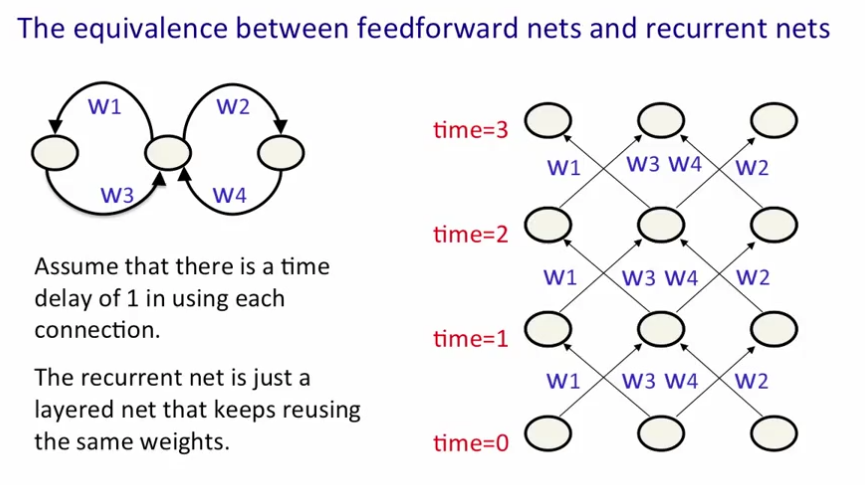
\includegraphics[scale=0.6]{sections/7/layered.png}
	\end{center}

	\subsubsection{Reminder: Backpropagation with weight constraints}
	\item It is easy to modify the backprop alg to incorporate linear constraints between the weights
	\item We compute the gradients as usual, and then modify the gradients so that they satsify the constraints
	\begin{itemize}
		\item To constrain: $w_1 = w_2$
		\item We need: $\delta w_1 = \delta w_2$
		\item compute: $\frac{\partial E}{\partial w_1}, \frac{\partial E}{\partial w_2}$
		\item use $\frac{\partial E}{\partial w_1}+\frac{\partial E}{\partial w_2}$ for $w_1$ and $w_2$
	\end{itemize}
	\item So if the weights started off satisfying constraints, they will continue too

	\subsubsection{Backpropagation through time}
	\item We can think of the recurrent net as a layered, feed-forward net with shared weights and then train the feed-forward net with weight constraints
	\item Training algorithm in the time domain
	\begin{itemize}
		\item Forward pass builds up activities at each time step
		\item Backward pass peels activities off stack and computes error derivatives at each time step
		\item Add together the derivatives at all the different times for each weight
	\end{itemize}

	\item We need to specify the initial activity state of all the hidden and ouput units
	\begin{itemize}
		\item We could fix these initial states to have some default value like 0.5.
		\item But it is better to treat the initial states as learned parameters
		\item We learn them in the same way we learn the weights
		\begin{itemize}
			\item Start off with an initial guess for the initial states
			\item At the end of each training sequence, backpropagate through time all the way to the intial states to get the gradient of the error function with respect to each inital state
			\item Adjust initial states by negative gradient
		\end{itemize}
	\end{itemize}

	\subsubsection{Providing input to recurrent networks}
	\begin{itemize}
		\item Several options:
		\begin{itemize}
			\item Specify the input states of all the units
			\item Specify the initial states of a subset of units
			\item Specify the states of the same subset of the units at every time step (natural way to model most sequential data; e.g., of the previous figure the first column of neurons)
		\end{itemize}

		\item We can specify targets in several ways too:
		\begin{itemize}
			\item Desired final activities of all the units
			\item 
		\end{itemize}
	\end{itemize}
\end{itemize}